\section{Evaluation}
In this section, the implementation details of the benchmarks are provided, as well as the selected datasets, and GPU architecture details that affect the result.

\subsection{String matching}
GPU-accelerated string matching frequently appears in GPU-based data\-bases, file carving~\cite{DataCarving,GPU-carving} that stands for extracting files from raw data in a field of cyber forensics, and intrusion detection~\cite{GPU-IDS}. Thus such a problem has a huge practical interest. Substrings could be considered static and subjected to partial evaluation.

\subsubsection{Na\`ive single substring matching}\label{naive-single}
Na\`ive algorithm operates on a \emph{subject} string and a \emph{pattern}, iteratively comparing each symbol of the pattern with the symbols of each substring of the subject string of size equal to the size of the pattern. The algorithm is inherently data-parallel: such substrings could be traversed separately, each in their thread. Further, such a traversal provides a rather optimal  global memory access pattern, since adjacent threads would access addresses of adjacent substrings. There exist an opportunity for optimization, since at one moment all threads in a warp access the same symbol of the pattern (and distinct symbols of the subject string), thus the pattern could be placed in constant memory to speed up the performance.

%<3 pushishku <3
 
There is a \emph{KMP} test for optimizers like partial evaluator, intended to check whether they correctly reduce static computations. 
Partial evaluation is able to reduce a na\`ive single substring matching, though properly rewritten, to something very like Knuth--Morris--Pratt algorithm~\cite{KMP-Danvy}, which uses a prefix function to recover from a mismatch, thus being linear with respect to the subject string.
When a mismatch occurs, it is known that all previous symbols of the pattern match the ones of the substring of the subject string up to the point of mismatch. 
In order to simulate a prefix function at the mismatch point, the pattern could be matched against itself up to this point, searching for the largest prefix being a suffix as well.
Since the pattern is static and matched against itself, this computation is fully static and could be performed at specialization time.
Porting this approach to GPU and Impala, and applying partial evaluation at runtime indeed produces a KMP-like program\footnote{\url{https://github.com/Tiltedprogrammer/spec/blob/master/kmp.dump}\\ (last accessed date: 30.05.2020)}. Thus, making the used partial evaluator sound in a sense. The KMP algorithm itself is hard to partially evaluate since the already matched piece of the pattern that drives the search through the backtracking table is fully dynamic.

However, such an approach is far less data parallel as well as KMP. The subject string should be divided into interleaved chunks, each assigned to a different thread. Such parallelization has a far worse access pattern since each thread accesses strided addresses of the subject string. However, in practice, such an access pattern occurs when the search is performed across different subject strings, where each thread operates on a specific string\footnote{\url{https://github.com/NVIDIA/nvstrings} (last accessed date: 30.05.2020)}

A na\`ive single substring matching could be also specialized by simply unrolling the traversal, that does not hurt the parallelization. The evaluation of these approaches is presented in figure~\ref{fig:kmp_test}.

\begin{figure}
    \centering
    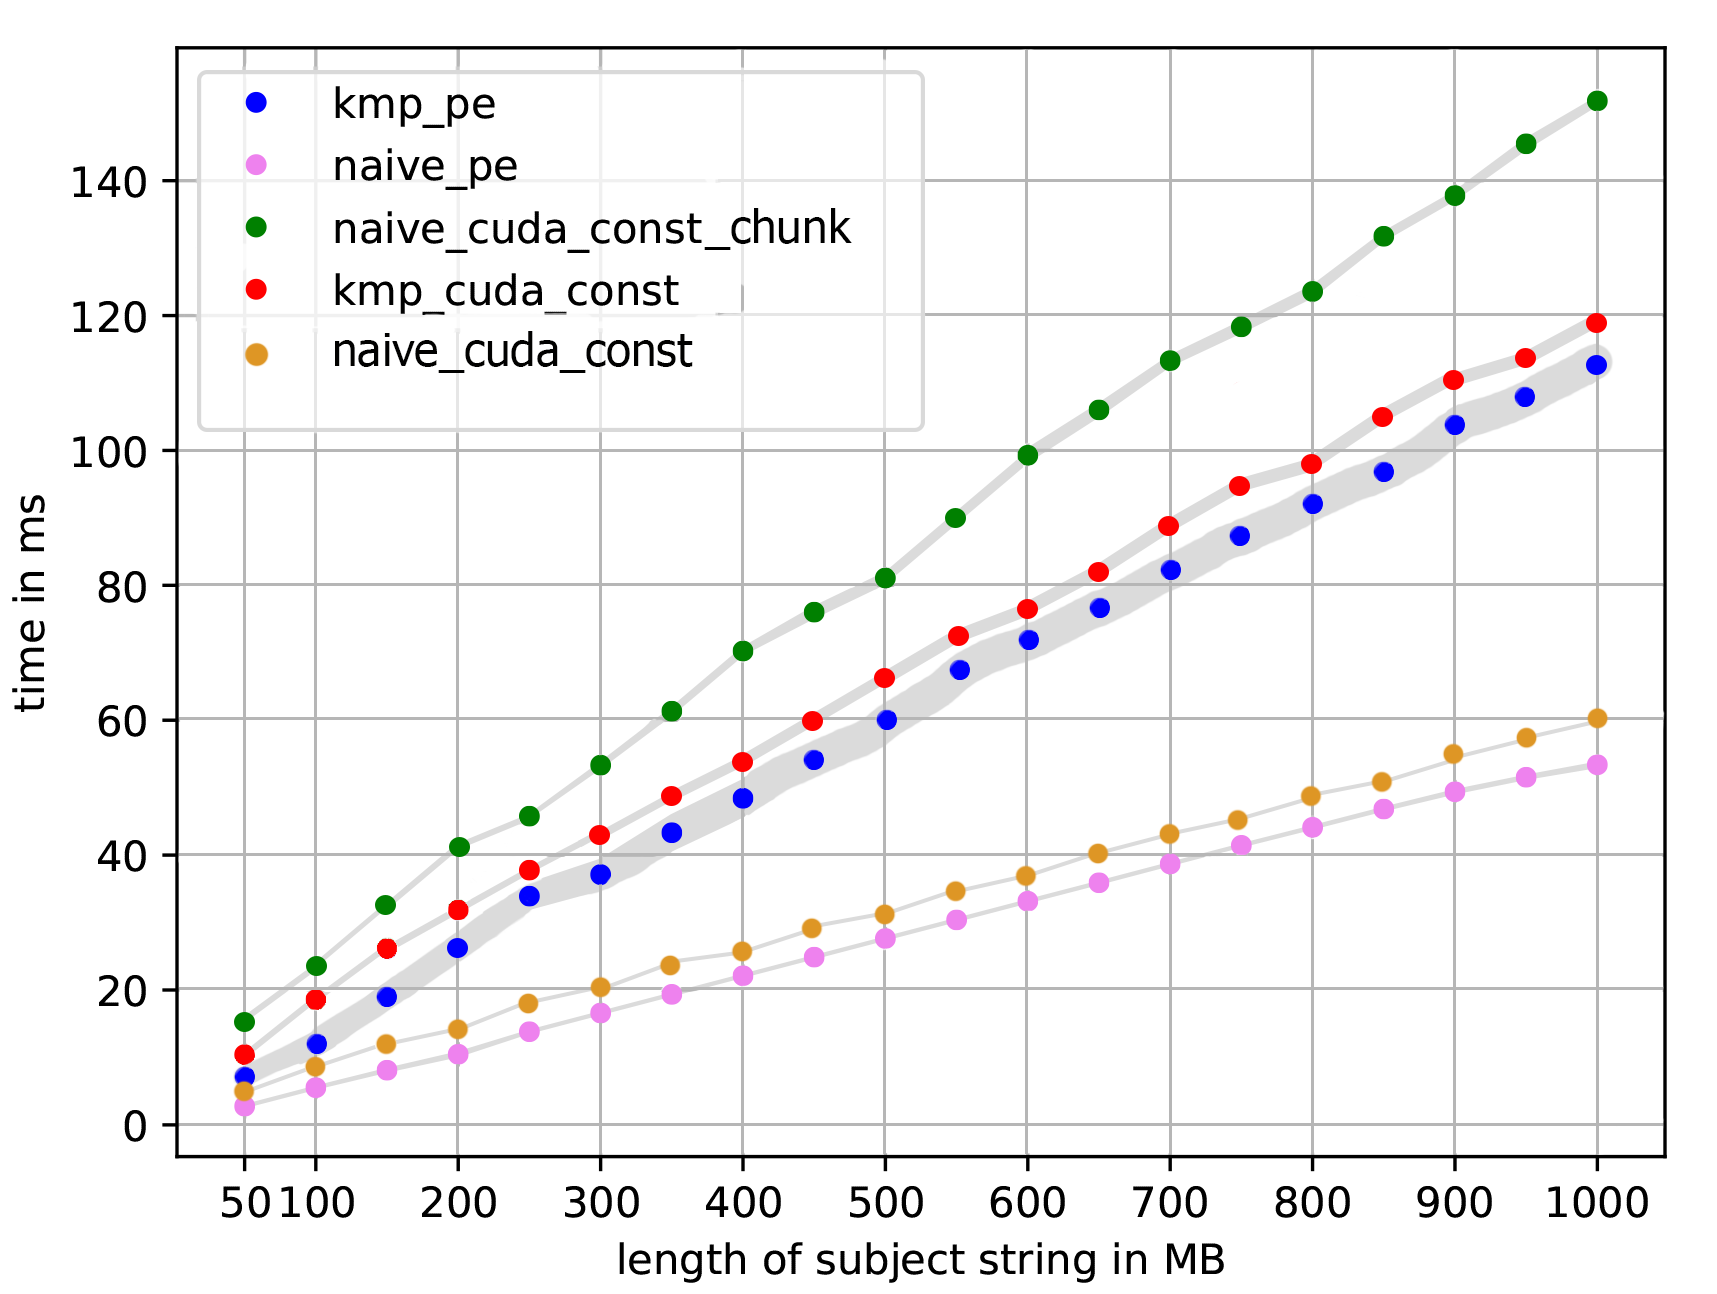
\includegraphics{figures/KMP_TEST.png}
    \caption{Na\`ive single substring matching}
    \label{fig:kmp_test}
\end{figure}

The current recursive implementation of the partial evaluator does not handle well the KMP test with patterns of more than 16 bytes in length. Thus, for the evaluation, a set of uniformly randomized 50 patterns\footnote{Enough for the divergence not to affect deviation so much.} from two-characters alphabet has been taken, satisfying that restriction. The subject string has been also randomly generated from the same alphabet. The standard deviation is shown in gray regions.
The KMP algorithm obtained by partial evaluation (\emph{kmp\_pe}), KMP algorithm implemented with CUDA, utilizing constant memory to store the backtrack table and the pattern (\emph{kmp\_cuda\_const}), na\`ive algorithm in CUDA with chunk-based parallelization (\emph{naive\_cuda\_const}), naive\`ive algorithm in CUDA with char-based parallelization and its partially evaluated version, that embeds the pattern into the code through unrolling the traversal, are compared. The figure grounds the success of the KMP test and shows that data embedding does not give any significant improvements: the difference between embedded and not embedded versions are mainly due to the reduced amount of address computations and loop overhead. The char-based parallel version is at the bottom due to a better memory access policy.

\subsubsection{Data embedding}\label{data_embedding}
Partial evaluation for the scenario above performed the transformation similar to the one in listing~\ref{code:kmp_spec}. While the load/store speed comparison for memory spaces is well described~\cite{TeslaT4Bench}, e.g. non-conflicting constant load is faster than L1 cache hit, the behavior of such embedded data is unspecified, but could be deduced as follows. All the arguments of assembly instructions should be put into registers, even the embedded ones, e.g. NVIDIA profiler\footnote{\url{https://developer.nvidia.com/nsight-visual-studio-edition} (last accessed date: 30.05.2020)} is able to tell how much of registers is required to perform an instruction: \lstinline{MOV R1 0x62} requires two registers, thus embedded data is eventually ending up in them. Yet, it is unclear from what memory space the embedded data is being put. The mini benchmark from listing~\ref{code:mem_bench} measures the number of cycles required to perform an addition operation \lstinline{add.u32} with one of the arguments passed via embedded value or via constant memory, lines 9 and 13. Given such a benchmark, the version with the value embedded performs 10 times faster: 42 cycles versus 430 on a constant cache miss. If the constant cache is firstly warmed up, the latency becomes 42 cycles and is the same for both instructions. Thus, embedded values are more likely to be accessed via instruction memory, since the instructions are prefetched and would outperform constant memory access under cache misses. Notably, when embedding, a partial evaluator is able to generate a more effective instruction, e.g. shift instead of division, which takes more than 10 instructions on GPU, while shift requires only one.

\begin{code}[language=C, caption=Memory benchmark,label=code:mem_bench,escapechar=!]
__constant__ int mini_array [2];

__global__ void dummy_kernel(int* dst,int* clocks){
    
    int i;
    int start,stop;
    
    asm volatile("mov.u32 %0, %%clock;": "=r"(start) :: "memory");
    asm volatile(
                 "add.u32 %0, %1, !\colorbox{yellow}{12}!;\n\t"
                 :"=r"(i) :"r"(i): "memory");
    // vs
    asm volatile(
                 "add.u32 %0, %1,!\colorbox{yellow}{\%2}!;\n\t"
                 :"=r"(i) :"r"(i),!\colorbox{yellow}{"r"(mini\_array[0]}!: "memory");
    asm volatile("mov.u32 %0, %%clock;": "=r"(stop) :: "memory");
}
\end{code}

\begin{code}[language=C,caption=KMP partial evaluation,label=code:kmp_spec,escapechar=!]
    //kmp_cuda_const
LDC R0, !\colorbox{yellow}{c[0x3][R0]}! //loads pattern's character from constant memory into register
    //...//
LDG R12, [R2] //loads subject's character from global memory
ISETP.NE.AND P0, !\colorbox{yellow}{R0}!, R12 // compares
    //..//
LDC R4, c[0x3][R2] // in case of mismatch goto position in backtrack table

    //kmp_pe
LDG R12, [R2] //loads subject's character from global memory
    //    ...
ISETP.NE.AND P0, R12, !\colorbox{yellow}{0x61}! // pattern's char is put right into the instruction
\end{code}

\subsubsection{Na\`ive multiple substring matching}\label{nmsm}

\begin{figure}
    \centering
    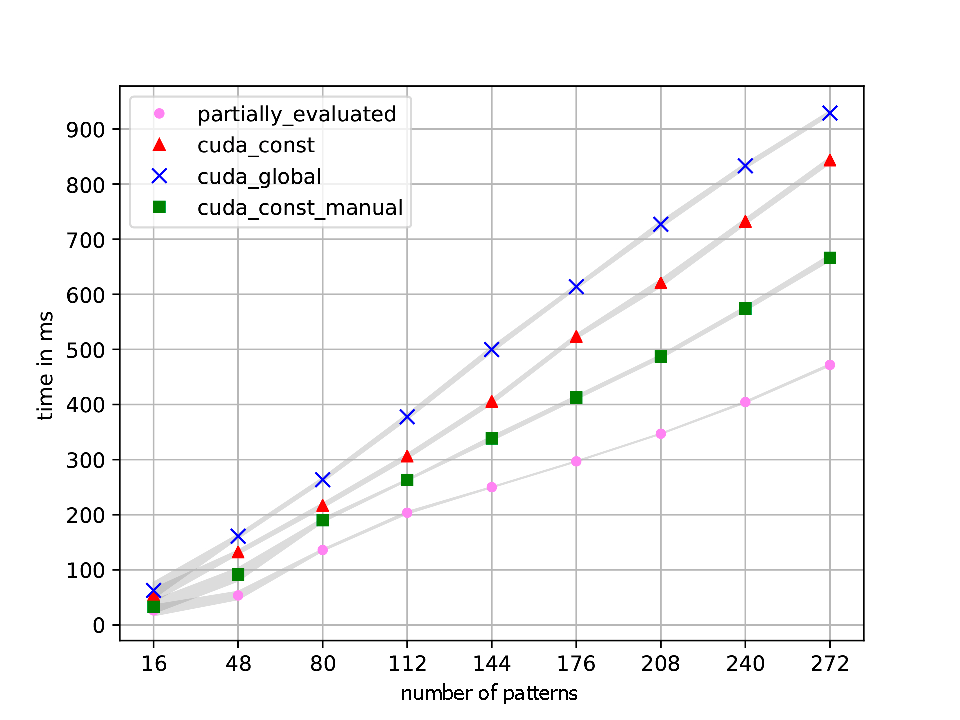
\includegraphics{figures/PredDefendNaiveSearch.pdf}
    \caption{Na\`ive multiple substring matching}
    \label{fig:naive_multy}
\end{figure}
The core of the algorithm is the same as the one of~\ref{naive-single} with the addition that a set of patterns is traversed against the substring. Since a set of patterns is traversed, their sizes are needed to be accessed, in order to be able to determine the border between the patterns. Constant memory could be utilized to store the sizes and the patterns, since threads of a warp access the same size and the same symbol of the pattern. Partially evaluating the algorithm with respect to the patterns, allows to fully reduce all the memory accesses to the sizes, which are numerous when the subject string is huge. Partial evaluation is achieved through loop unrolling for the sizes and the patterns. The results of this benchmark are presented in figure~\ref{fig:naive_multy}.

The dataset is from the intrusion detection area, which is common for multiple pattern matching problems~\cite{Aho-Corasick}. The subject string is 500MB \emph{tcpdump} from \emph{Botnet} dataset~\cite{Ring_2019}. The patterns are extracted from \emph{Snort V3}\footnote{\url{https://www.snort.org/downloads} (last accessed date: 30.05.2020)} rules, which are the patterns containing malicious traffic. The same set of patterns has been run over 30 times taking the average. The gray area represents the standard deviation.

\emph{Cuda\_global} is the implementation with global memory for storing the sizes and the patterns, while \emph{cuda\_const} uses constant memory for this. As it could be seen, the partially evaluated version is at the very bottom being 2x faster than the version with constant memory. \emph{cuda\_const\_manual} is the implementation, where all size accesses have been reduced manually, using a CUDA JIT compiler\footnote{https://github.com/NVIDIA/jitify}. It is slower than the partially evaluated version due to the reasons related to CUDA compiler implementation. In this case, provided the patterns embedded into the code, the compiler is able to produce a more efficient code from listing~\ref{code:vs}, considering the number of instructions. It could be tempting to embed data of size exceeding a constant memory pool of 64 KB into code, provided that such access could be even faster. First, CUDA limits the maximum number of instructions that could be put into a module by 512 million. Second, compilation time begins to matter for relatively huge embedded data, e.g. 272 patterns are \~5KB in size and compilation took several minutes.

\begin{code}[language=C,caption=Cuda\_const\_manual vs partially\_evaluated,label=code:vs,escapechar=!]
    //Cuda_const_manual

IMAD.MOV.U32 R8, RZ, RZ, R4 
ULDC.64 UR4, c[0x0][0x160]
IMAD.MOV.U32 R9, RZ, RZ, R3
LDG.E.U8.SYS R8, [R8.64+UR4+0x1] // load subject's character
ULDC.U8 UR4, c[0x3][0x1] //load pattern's character
ULOP UR4, UR4, 0xff, URZ, 0xc0
IMAD.U32 R11, RZ, RZ, UR4
PRMT R11, R11, 0x9910,RZ
PRMT R12, R8, 0x9910,RZ
ISETP.NE.AND P0, PT, R12, R11, PT //compare

    //partially_evaluated

IMAD.MOV.U32 R6, RZ, RZ, R2 
ULDC.64 UR6, c[0x0][0x160] 
IMAD.MOV U32 R7, RZ, RZ, R5 
LDG.E.U8.SYS R6, [R6.64 + UR6+0x1] // load subject's character
PRMT R8, R6, 0x9910, RZ
ISETP.NE.AND P0, PT, R8, 0x42, PT //compare

\end{code}

\subsubsection{Aho-Corasick matching}
Aho-Corasick is a time efficient algorithm for multiple string pattern matching~\cite{Aho-Corasick} and based on suffix tree and a failure transition table. However, a failure transition table becomes redundant by switching to GPU, since a simple suffix tree traversal per thread for each position in the subject string appear to be more efficient~\cite{PFAC}. The parallel Aho-Corasick first construct a transition table where final states have numbers less than the starting state, to reduce memory accesses for checking whether the state is final or not. The table is stored in global memory and each thread traverses the table taking a subject string character from shared memory. The benchmark and the implemented algorithms are presented in figure~\ref{fig:my_corasick}. The dataset used is the same as in~\ref{nmsm}. \emph{Cuda\_corasick\_lib} is the implementation of this algorithm\footnote{https://github.com/pfac-lib/PFAC} taken from~\cite{PFAC}. The transition table is often sparse and could be embedded into the code during partial evaluation using static binding of dynamic variables~\cite{Jones1993} avoiding empty entries, \emph{corasick\_pe} is the implementation of this approach. \emph{Naive\_pe} is the algorithm from~\ref{nmsm} utilizing shared memory. \emph{Cuda\_corasick\_pe} is the implementation, where a pattern set specific interpreter for the transition table is generated. The interpreter represents a sequence of code-embedded conditional statements to traverse the suffix tree.


\begin{figure}[h!]
    \centering
    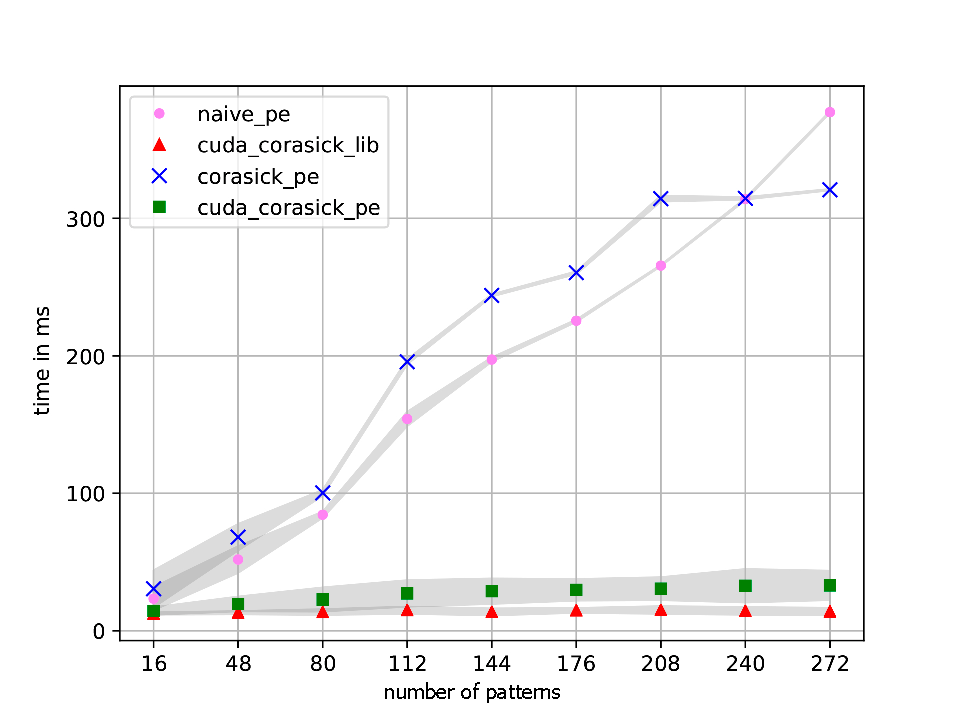
\includegraphics{figures/PredDefendNaiveSearchorasick(eng).pdf}
    \caption{Aho-Corasick matching}
    \label{fig:my_corasick}
\end{figure}

Static binding is a traversal of statically known possible values of a dynamic parameter in a bunch of condition statements. In this case, such an approach induces more thread divergence, e.g. 6 times if compared to \emph{cuda\_corasick\_lib}, which drastically decreases the performance of a GPU application. The interpreter approach has better divergence behavior but still diverges twice as much as \emph{cuda\_corasick\_lib}. So, given that global memory access latency even on L1 cache hit is more than the one for embedded data, the static binding approach that could work well on a CPU has a poor performance when a GPU is used, and even if interpretative implementation is near, such an embedding also does not provide any performance benefit.


\subsection{Convolutional filtering}

\begin{figure}[h!]
    \centering
    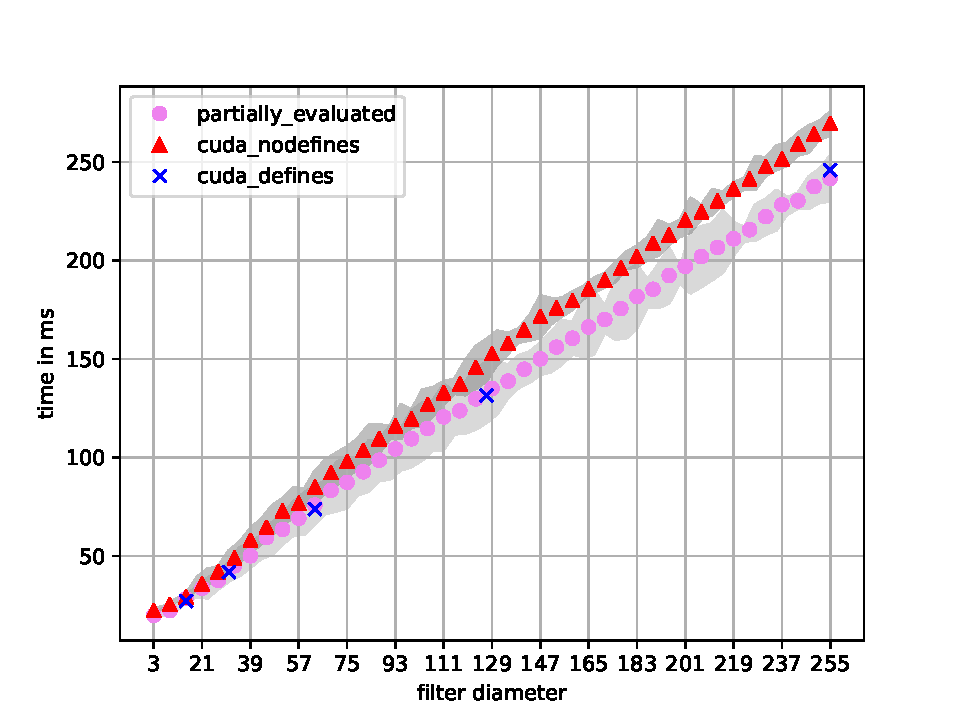
\includegraphics{figures/separable_convolution_diploma.pdf}
    \caption{Separable convolution}
    \label{fig:convolution}
\end{figure}
Convolutional filtering is a matrix dot product frequently used in image processing~\cite{chetlur2014cudnn}. Basically, there are a huge subject matrix and a small filter matrix, and each submatrix of the subject matrix is dot producted with the filter matrix.
Since the filter is small and is static, the convolution operation could be partially evaluated with respect to the filter.
A partial evaluation for a 2-D separable\footnote{1-D filter could be applied first to rows and then to columns.} convolutional filtering has been performed in~\cite{OnlinePe}, targeting different hardware, however, the described filter is a rewritten modification of the reference filter, thus the obtained speed-up is not achieved by means of partial evaluator solely, and is used to demonstrate the facilities of the Impala language.

\subsubsection{Separable convolution}

A separable convolutional filter has been implemented in CUDA and Impala~\cite{CudaConv}. It operates on a 2-D array in global memory with threads organized in $32 x 16$ blocks, where each thread convolves 8 elements. Shared memory is utilized to store the big area for convolution with a block and the required borders. Since the filter is read-only and accessed equally by all the threads, it is stored in constant memory. Elements that fall away the borders of the 2-D subject array are assigned zeroes. There are two device kernels to perform a convolution: one convolves the rows and the other convolves the columns with the shared memory padded enough to not cause bank conflicts when accessing column elements.

\begin{code}[language=C,label=code:conv,caption=Convolution partial evaluation,escapechar=!]
//cuda_defines
LDS.U R16, [R2 + 0x38] //load from shared
FFMA R17, R10, !\colorbox{yellow}{c[0x3][0x1dc]}! R17 //float multiply add

//partially_evaluated
LDS.U R16, [R2 + 0x38] //load from shared
FFMA R17, R10, !\colorbox{yellow}{42}! R17 //float multiply add
\end{code}

The convolution itself is a dot product of two vectors of filter size. Since the size is known, this cycle could be unrolled with the filter being embedded. %In~\cite{OnlinePe} the partial evaluator generated different convolve functions for regions of the 2-D array that are near the borders (assigned with zeroes), and ones that are not, reducing the number of conditional statements. However, this is not portable on a GPU, since which thread block would operate on a borders area is a device kernel runtime information and thus is fully dynamic and could not be exploited. In
Such an unroll could be also performed by means of C++ templates or macros, by creating a dedicated device kernel for a specific filter size and dynamically dispatching the appropriate kernel for input data. The results of the benchmark are depicted in figure~\ref{fig:convolution}. The subject 2-D array is 1GB randomly generated, the filters are randomly generated for each diameter. The average has been taken for each filter size from 30 runs. The gray area is the standard deviation. \emph{Cuda\_nodefines} is the implementation with the dot product not unrolled, \emph{cuda\_defines} leverages macros to unroll the product, \emph{partially\_evaluated} leverages partial evaluation. Unrolled versions are at the bottom since they reduce the loop overhead. Unrolled version perform equally due to the code generated by the compiler as in listing~\ref{code:conv} which has been shown to be executed in the same number of cycles in~\ref{data_embedding}.

\subsection{Discussion}

While data embedding by means of partial evaluation achieves the same performance as constant memory access, given that no access instructions had been reduced, there are cases when it outperforms due to the reasons internal to the compiler.
Thus, partial evaluation could be a way to automate constant memory management and even speed up the performance.
Since the performance is compiler specific, which is further device-specific, there is a need to investigate the compiler which is publicly unspecified, and at the moment of writing there is a lack of tools for that.
Also, partial evaluation performance is scenario- specific, hence other scenarios should be investigated as well.
Finally, guidelines of developing a program that is amenable to partial evaluation~\cite{Jones1993} could be extended to explicitly multithreaded programs such as CUDA kernels, or the semantics of the intermediate representation could consider the multithreaded environment.
However, these questions are beyond the scope of the work.


%The runtime compilation overhead could be estimated 
% Unlike possible fully dynamic thread divergence, induced by partial evaluation, i.e. divergence could differ in different runs depending on the data, compiler is static. Thus, in this case the possible performance could be as well statically estimated prior to running the kernel

